\newcommand{\downloaderTagResultsAucTable}{
    \begin{table}[H]
        \centering
        \begin{tabular}{|p{2,8cm}||p{2,8cm} p{2,8cm} p{2,8cm}|}
            \hline
            Downloader Tag & ALOHA & Joint Embedding & Proposed Model \\
            \hline
            AUC-ROC & 0.973$\pm$0.003 & 0.977$\pm$0.002 & \textBF{0.977$\pm$0.001} \\
            \hline
        \end{tabular}
        \caption{AUC-ROC (Area Under Curve) of the different models for the \textbf{Downloader Tag} prediction task. Results were aggregated over \textBF{3} training runs with different weight initializations and minibatch orderings. Best results are shown in \textbf{bold}.} \label{tab:downloaderTag_auc}
    \end{table}
}

\newcommand{\downloaderTagResultsAtFprTable}{
    \begin{center}
        \begin{longtable}[c]{|p{3,2cm}||p{1,8cm} p{1,8cm} p{1,8cm} p{1,8cm} p{1,8cm}|}
            \hline
            Downloader Tag & \multicolumn{5}{c|}{{FPR}} \\
            & $10^{-5}$ & $10^{-4}$ & $10^{-3}$ & $10^{-2}$ & $10^{-1}$ \\
            \hline
            \endfirsthead

            \caption*{\raggedright ...continued from previous page} \\
            \hline
            Downloader Tag & \multicolumn{5}{c|}{\textbf{FPR}} \\
            & $10^{-5}$ & $10^{-4}$ & $10^{-3}$ & $10^{-2}$ & $10^{-1}$ \\
            \hline
            \endhead

            \caption*{\raggedleft ...continued on next page} \\
            \endfoot

            \caption{Mean and standard deviation results (TPR, Accuracy, Recall, Precision and F1-Score) of the different models for the \textbf{Downloader Tag} prediction task at different \textbf{FPR}s (\textit{False Positive Rates}). Results were aggregated over \textBF{3} training runs with different weight initializations and minibatch orderings. Best results are shown in \textbf{bold}. Under \textbf{TPR} results are also presented the percentage reduction in mean detection error and in ROC curve standard deviation introduced by the \textit{Proposed Model} with respect to both \textit{ALOHA} model and \textit{Joint Embedding}.} \label{tab:downloaderTag_results_at_fpr} \\
            \endlastfoot

            \multicolumn{6}{|c|}{\textbf{TPR}} \\
            \hline
            ALOHA & \textBF{0.227$\pm$0.103} & \textBF{0.439$\pm$0.061} & 0.550$\pm$0.045 & 0.619$\pm$0.020 & 0.942$\pm$0.002 \\
            Joint Embedding & 0.130$\pm$0.031 & 0.296$\pm$0.071 & 0.543$\pm$0.044 & 0.638$\pm$0.008 & 0.957$\pm$0.003 \\
            Proposed Model & 0.162$\pm$0.032 & 0.319$\pm$0.016 & \textBF{0.589$\pm$0.007} & \textBF{0.664$\pm$0.008} & \textBF{0.960$\pm$0.006} \\
            \hline
            Error Reduction wrt \newline ALOHA & -8.4\% & -21.4\% & 8.7\% & 11.8\% & 31.0\% \\
            Error Reduction wrt \newline Joint Embedding & 3.7\% & 3.3\% & 10.1\% & 7.2\% & 7.0\% \\
            \hline
            Std Reduction wrt \newline ALOHA & 68.9\% & 73.8\% & 84.4\% & 60.0\% & -200.0\% \\
            Std Reduction wrt \newline Joint Embedding & -3.2\% & 77.5\% & 84.1\% & 0.0\% & -100.0\% \\
            \hline
            \multicolumn{6}{|c|}{\textbf{Accuracy}} \\
            \hline
            ALOHA & \textBF{0.935$\pm$0.009} & \textBF{0.953$\pm$0.005} & 0.961$\pm$0.004 & 0.959$\pm$0.002 & 0.904$\pm$0.000 \\
            Joint Embedding & 0.927$\pm$0.003 & 0.941$\pm$0.006 & 0.961$\pm$0.004 & 0.961$\pm$0.001 & \textBF{0.905$\pm$0.000} \\
            Proposed Model & 0.930$\pm$0.003 & 0.943$\pm$0.001 & \textBF{0.965$\pm$0.001} & \textBF{0.963$\pm$0.001} & 0.905$\pm$0.001 \\
            \hline
            \multicolumn{6}{|c|}{\textbf{Recall}} \\
            \hline
            ALOHA & \textBF{0.227$\pm$0.103} & \textBF{0.439$\pm$0.061} & 0.550$\pm$0.045 & 0.619$\pm$0.020 & 0.942$\pm$0.002 \\
            Joint Embedding & 0.130$\pm$0.031 & 0.296$\pm$0.071 & 0.543$\pm$0.044 & 0.638$\pm$0.008 & 0.957$\pm$0.003 \\
            Proposed Model & 0.162$\pm$0.032 & 0.319$\pm$0.016 & \textBF{0.589$\pm$0.007} & \textBF{0.664$\pm$0.008} & \textBF{0.960$\pm$0.006} \\
            \hline
            \multicolumn{6}{|c|}{\textbf{Precision}} \\
            \hline
            ALOHA & \textBF{0.999$\pm$0.000} & \textBF{0.997$\pm$0.000} & 0.980$\pm$0.002 & 0.850$\pm$0.004 & 0.462$\pm$0.001 \\
            Joint Embedding & \textBF{0.999$\pm$0.000} & 0.996$\pm$0.001 & 0.980$\pm$0.002 & 0.853$\pm$0.002 & 0.466$\pm$0.001 \\
            Proposed Model & \textBF{0.999$\pm$0.000} & \textBF{0.997$\pm$0.000} & \textBF{0.982$\pm$0.000} & \textBF{0.858$\pm$0.002} & \textBF{0.467$\pm$0.002} \\
            \hline
            \multicolumn{6}{|c|}{\textbf{F1 Score}} \\
            \hline
            ALOHA & \textBF{0.358$\pm$0.146} & \textBF{0.607$\pm$0.061} & 0.704$\pm$0.037 & 0.716$\pm$0.014 & 0.620$\pm$0.001 \\
            Joint Embedding & 0.229$\pm$0.049 & 0.452$\pm$0.083 & 0.698$\pm$0.037 & 0.730$\pm$0.006 & 0.627$\pm$0.001 \\
            Proposed Model & 0.277$\pm$0.046 & 0.483$\pm$0.018 & \textBF{0.736$\pm$0.006} & \textBF{0.749$\pm$0.006} & \textBF{0.628$\pm$0.003} \\
            \hline
        \end{longtable}
    \end{center}
}

\newcommand{\downloaderTagResultsSummaryTable}{
    \begin{table}[H]
        \centering
        \begin{tabular}{|p{3,2cm}||p{1,8cm} p{1,8cm} p{1,8cm} p{1,8cm} p{1,8cm}|}
            \hline
            \multicolumn{6}{|c|}{Downloader Tag (at FPR $=1\%$)} \\
            \hline
            Model & TPR & Accuracy & Precision & Recall & F1 score \\
            \hline
            ALOHA & 0.619$\pm$0.020 & 0.959$\pm$0.002 & 0.850$\pm$0.004 & 0.619$\pm$0.020 & 0.716$\pm$0.014 \\
            Joint Embedding & 0.638$\pm$0.008 & 0.961$\pm$0.001 & 0.853$\pm$0.002 & 0.638$\pm$0.008 & 0.730$\pm$0.006 \\
            Proposed Model & \textBF{0.664$\pm$0.008} & \textBF{0.963$\pm$0.001} & \textBF{0.858$\pm$0.002} & \textBF{0.664$\pm$0.008} & \textBF{0.749$\pm$0.006} \\
            \hline
        \end{tabular}
        \caption{Summary of the mean and standard deviation results of the different models for the \textbf{Downloader Tag} prediction task at \textbf{FPR} $=1\%$. Results were aggregated over \textBF{3} training runs with different weight initializations and minibatch orderings. Best results are shown in \textbf{bold}.} \label{tab:downloaderTag_result_summary}
    \end{table}
}

\newcommand{\downloaderTagRocAloha}{
    \begin{figure}[H]
        \vspace*{-0.5cm}
        \centering
        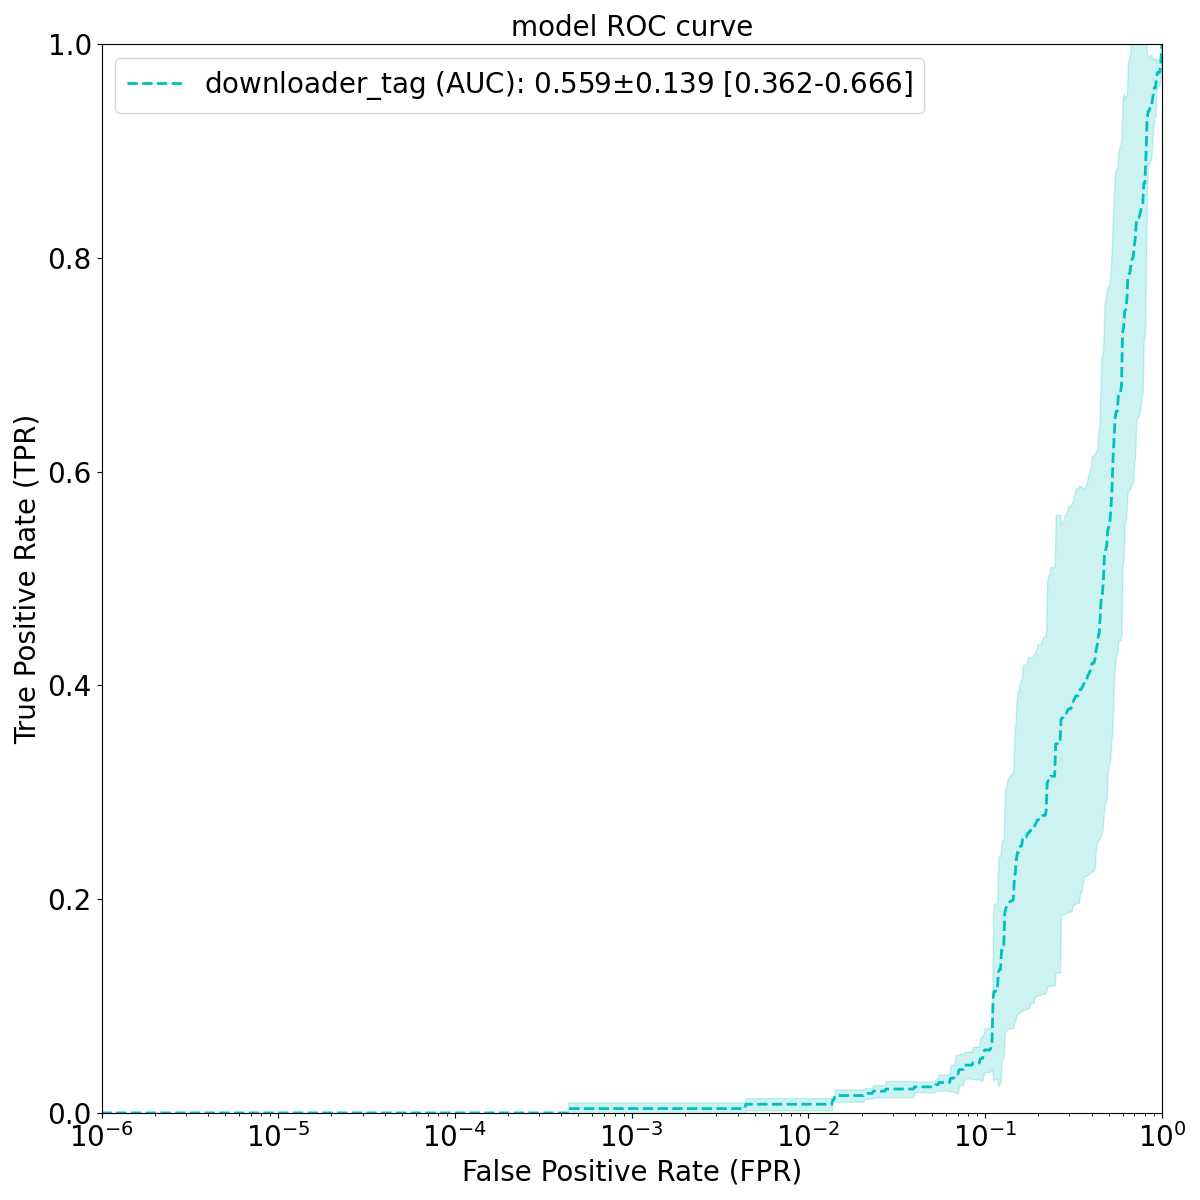
\includegraphics[width=0.6\textwidth]{./results/downloader_tag_roc_aloha.png}
        \vspace*{-0.2cm}
        \caption{ROC curve and AUC statistics of \textBF{ALOHA} model for the \textbf{Downloader Tag}. The line represents the \textit{mean} TPR at a given FPR, while the shaded region represents the \textit{standard deviation}. Statistics were computed over \textBF{3} training runs, each with random parameter initialization.}
        \label{fig:downloaderTagRocAloha}
    \end{figure}
}

\newcommand{\downloaderTagRocJointEmbedding}{
    \begin{figure}[H]
        \vspace*{-0.5cm}
        \centering
        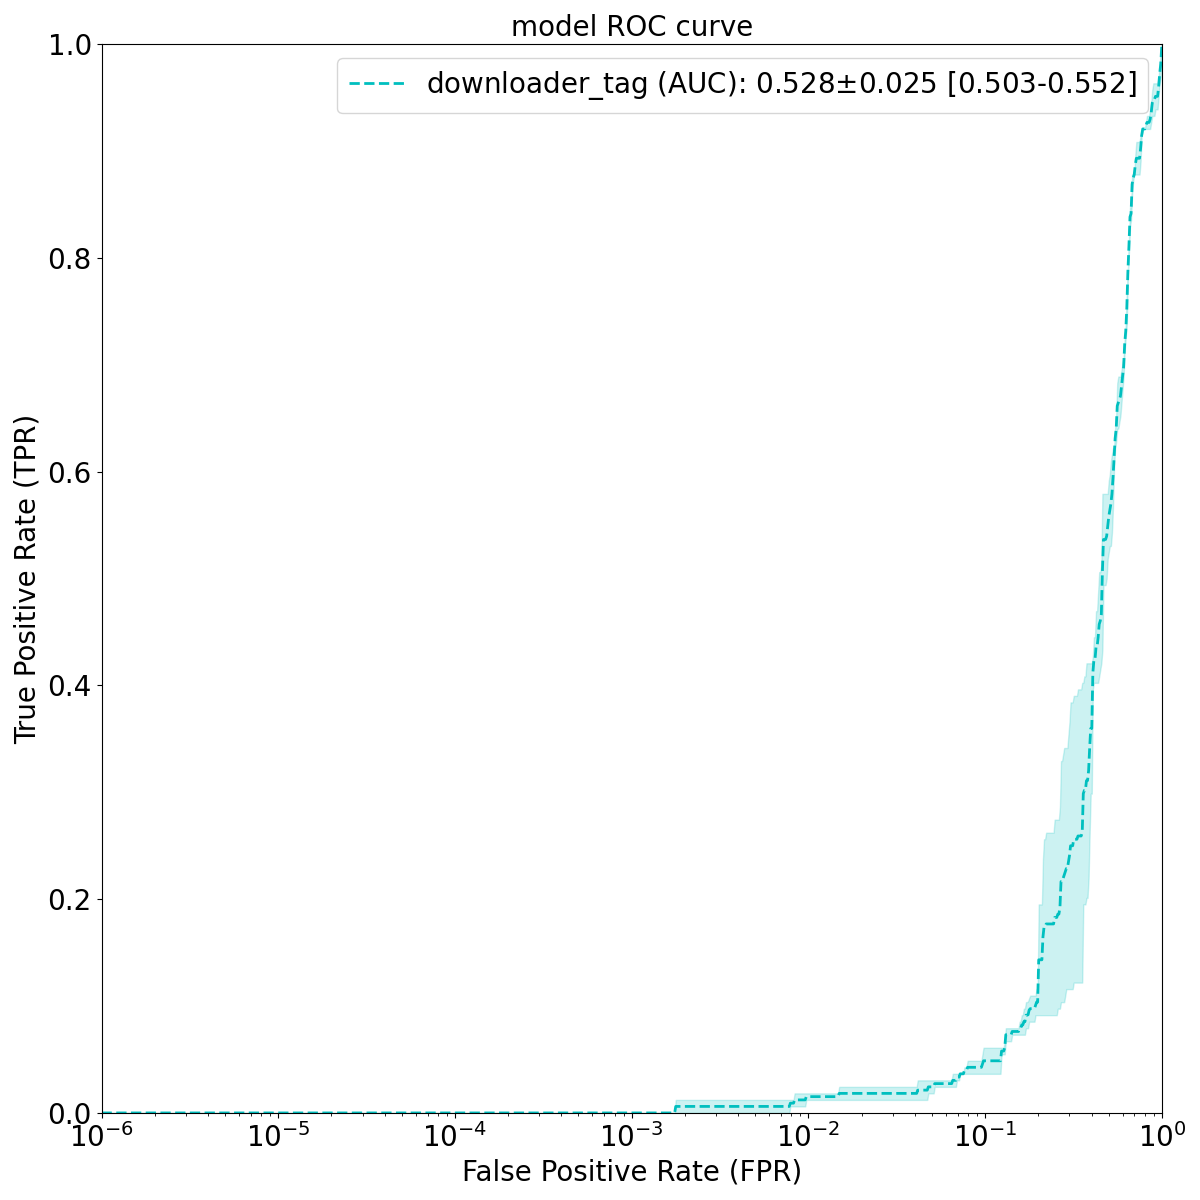
\includegraphics[width=0.6\textwidth]{./results/downloader_tag_roc_jointEmbedding.png}
        \vspace*{-0.2cm}
        \caption{ROC curve and AUC statistics of \textBF{Joint Embedding} model for the \textbf{Downloader Tag}. The line represents the \textit{mean} TPR at a given FPR, while the shaded region represents the \textit{standard deviation}. Statistics were computed over \textBF{3} training runs, each with random parameter initialization.}
        \label{fig:downloaderTagRocJointEmbedding}
    \end{figure}
}

\newcommand{\downloaderTagRocProposedMethod}{
    \begin{figure}[H]
        \vspace*{-0.5cm}
        \centering
        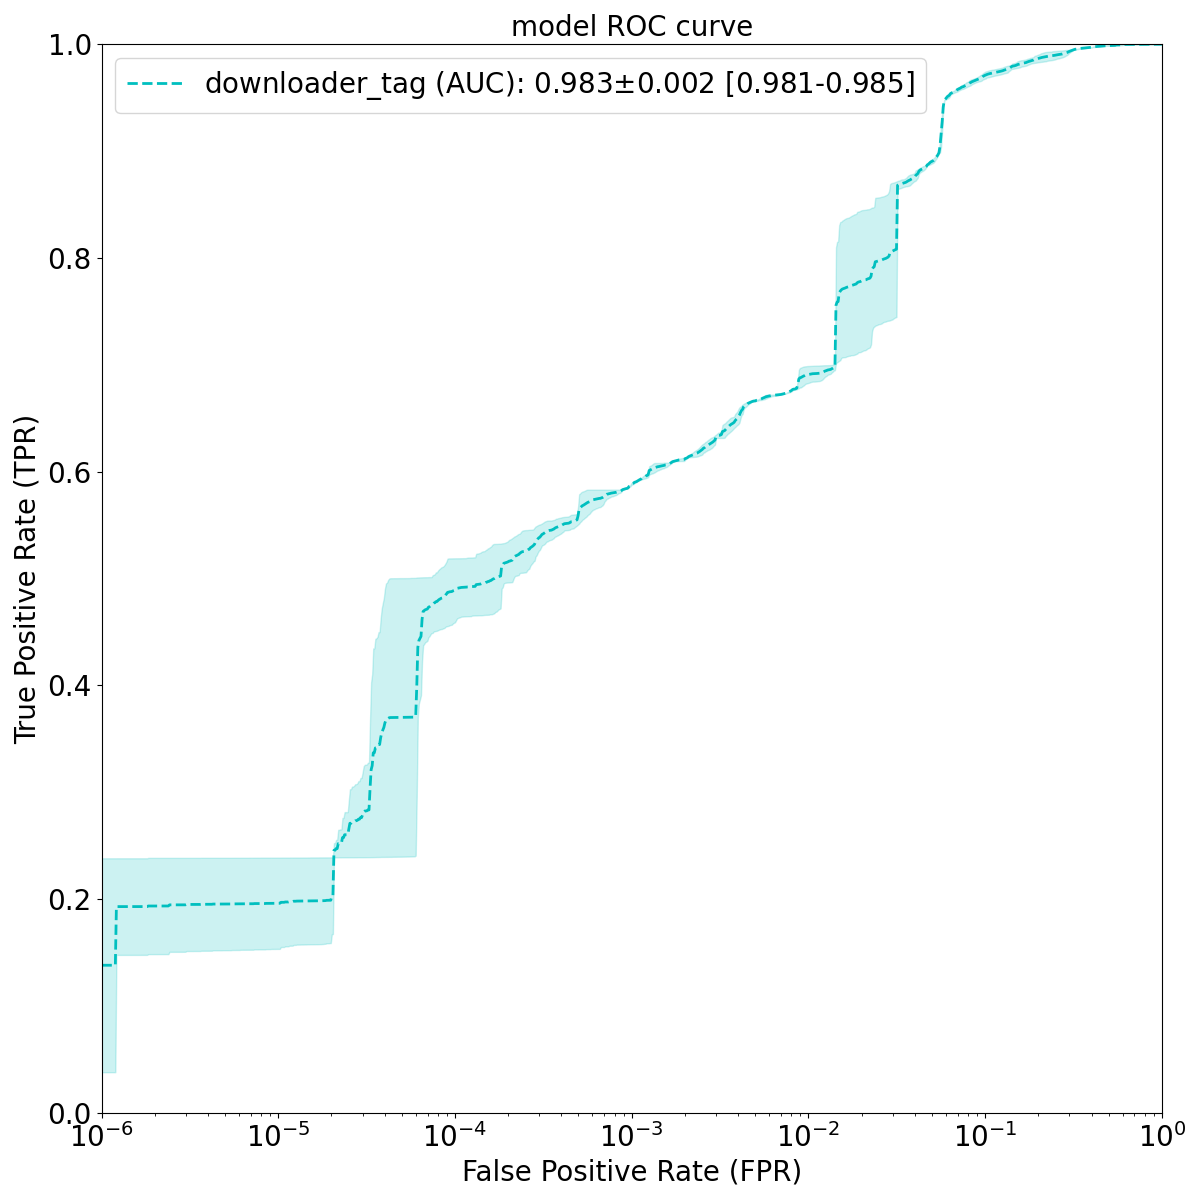
\includegraphics[width=0.6\textwidth]{./results/downloader_tag_roc_proposedModel.png}
        \vspace*{-0.2cm}
        \caption{ROC curve and AUC statistics of \textBF{Proposed Model} for the \textbf{Downloader Tag}. The line represents the \textit{mean} TPR at a given FPR, while the shaded region represents the \textit{standard deviation}. Statistics were computed over \textBF{3} training runs, each with random parameter initialization.}
        \label{fig:downloaderTagRocProposedModel}
    \end{figure}
}
